\chapter{Análisis complementario del proceso de \emph{infill}}
\label{app:visualizacion_infill}

Este anexo complementa el material de benchmarks del Anexo~\ref{app:benchmarks_complementario} con una lectura visual y estadística del proceso de \emph{infill}. El objetivo no es introducir nuevos resultados principales, sino mostrar con más detalle cómo el modelo sustituto participa en la selección secuencial de puntos y por qué las métricas predictivas y las métricas de optimización no siempre seleccionan el mismo modelo.

\section{Relación entre mejora predictiva y mejora del mínimo encontrado}
\label{app:relacion_mae_incumbent}

El Cuadro~\ref{tab:app_modelos_incumbent_mae} compara, para cada benchmark, el modelo con mayor mejora del mínimo encontrado frente al modelo con mayor mejora relativa del MAE. Esta comparación es relevante porque el objetivo de un ciclo de optimización por \emph{infill} no es necesariamente minimizar el error medio global del modelo sustituto, sino encontrar mejores valores de la función objetivo con un presupuesto limitado de evaluaciones.

\begin{table}[htbp]
\centering
\small
\caption[Mejora del incumbent frente a mejora del MAE]{Comparación entre el mejor modelo según mejora del mínimo encontrado y el mejor modelo según mejora relativa del MAE.}
\label{tab:app_modelos_incumbent_mae}
\renewcommand{\arraystretch}{1.15}
\begin{tabularx}{\textwidth}{@{}p{2.4cm} p{3.0cm} p{2.0cm} p{3.0cm} p{2.0cm}@{}}
\toprule
\textbf{Benchmark} & \textbf{Mejor modelo por mínimo encontrado} & \textbf{Mejora \emph{inc.}} & \textbf{Mejor modelo por MAE} & \textbf{Mejora MAE} \\
\midrule
Borehole & GP\_Linear & 0.720 & GP\_RBF\_ARD & 0.574 \\
Branin & GP\_Matern52\_ARD & 0.898 & GP\_RBF & 0.175 \\
Forrester & GP\_Matern52 & 0.737 & GP\_RBF & 0.281 \\
Hartmann6 & GP\_RBF & 0.434 & GP\_Linear & 0.466 \\
\bottomrule
\end{tabularx}
\end{table}
\FloatBarrier

En todos los benchmarks del Cuadro~\ref{tab:app_modelos_incumbent_mae}, el modelo que más reduce el error medio no coincide necesariamente con el modelo que consigue mayor mejora del mínimo encontrado. Este resultado justifica analizar por separado la calidad predictiva del modelo sustituto y la eficacia del proceso de búsqueda.

\section{Forrester como caso visual del mecanismo de \emph{infill}}
\label{app:forrester_visual}

Forrester se utiliza como caso visual porque es un benchmark unidimensional. Esta propiedad permite representar simultáneamente la función real, la media posterior del GP, la incertidumbre predictiva y los puntos observados. Por tanto, resulta adecuado para explicar de forma gráfica el papel de EI en la selección de nuevas evaluaciones.

\begin{figure}[htbp]
\centering
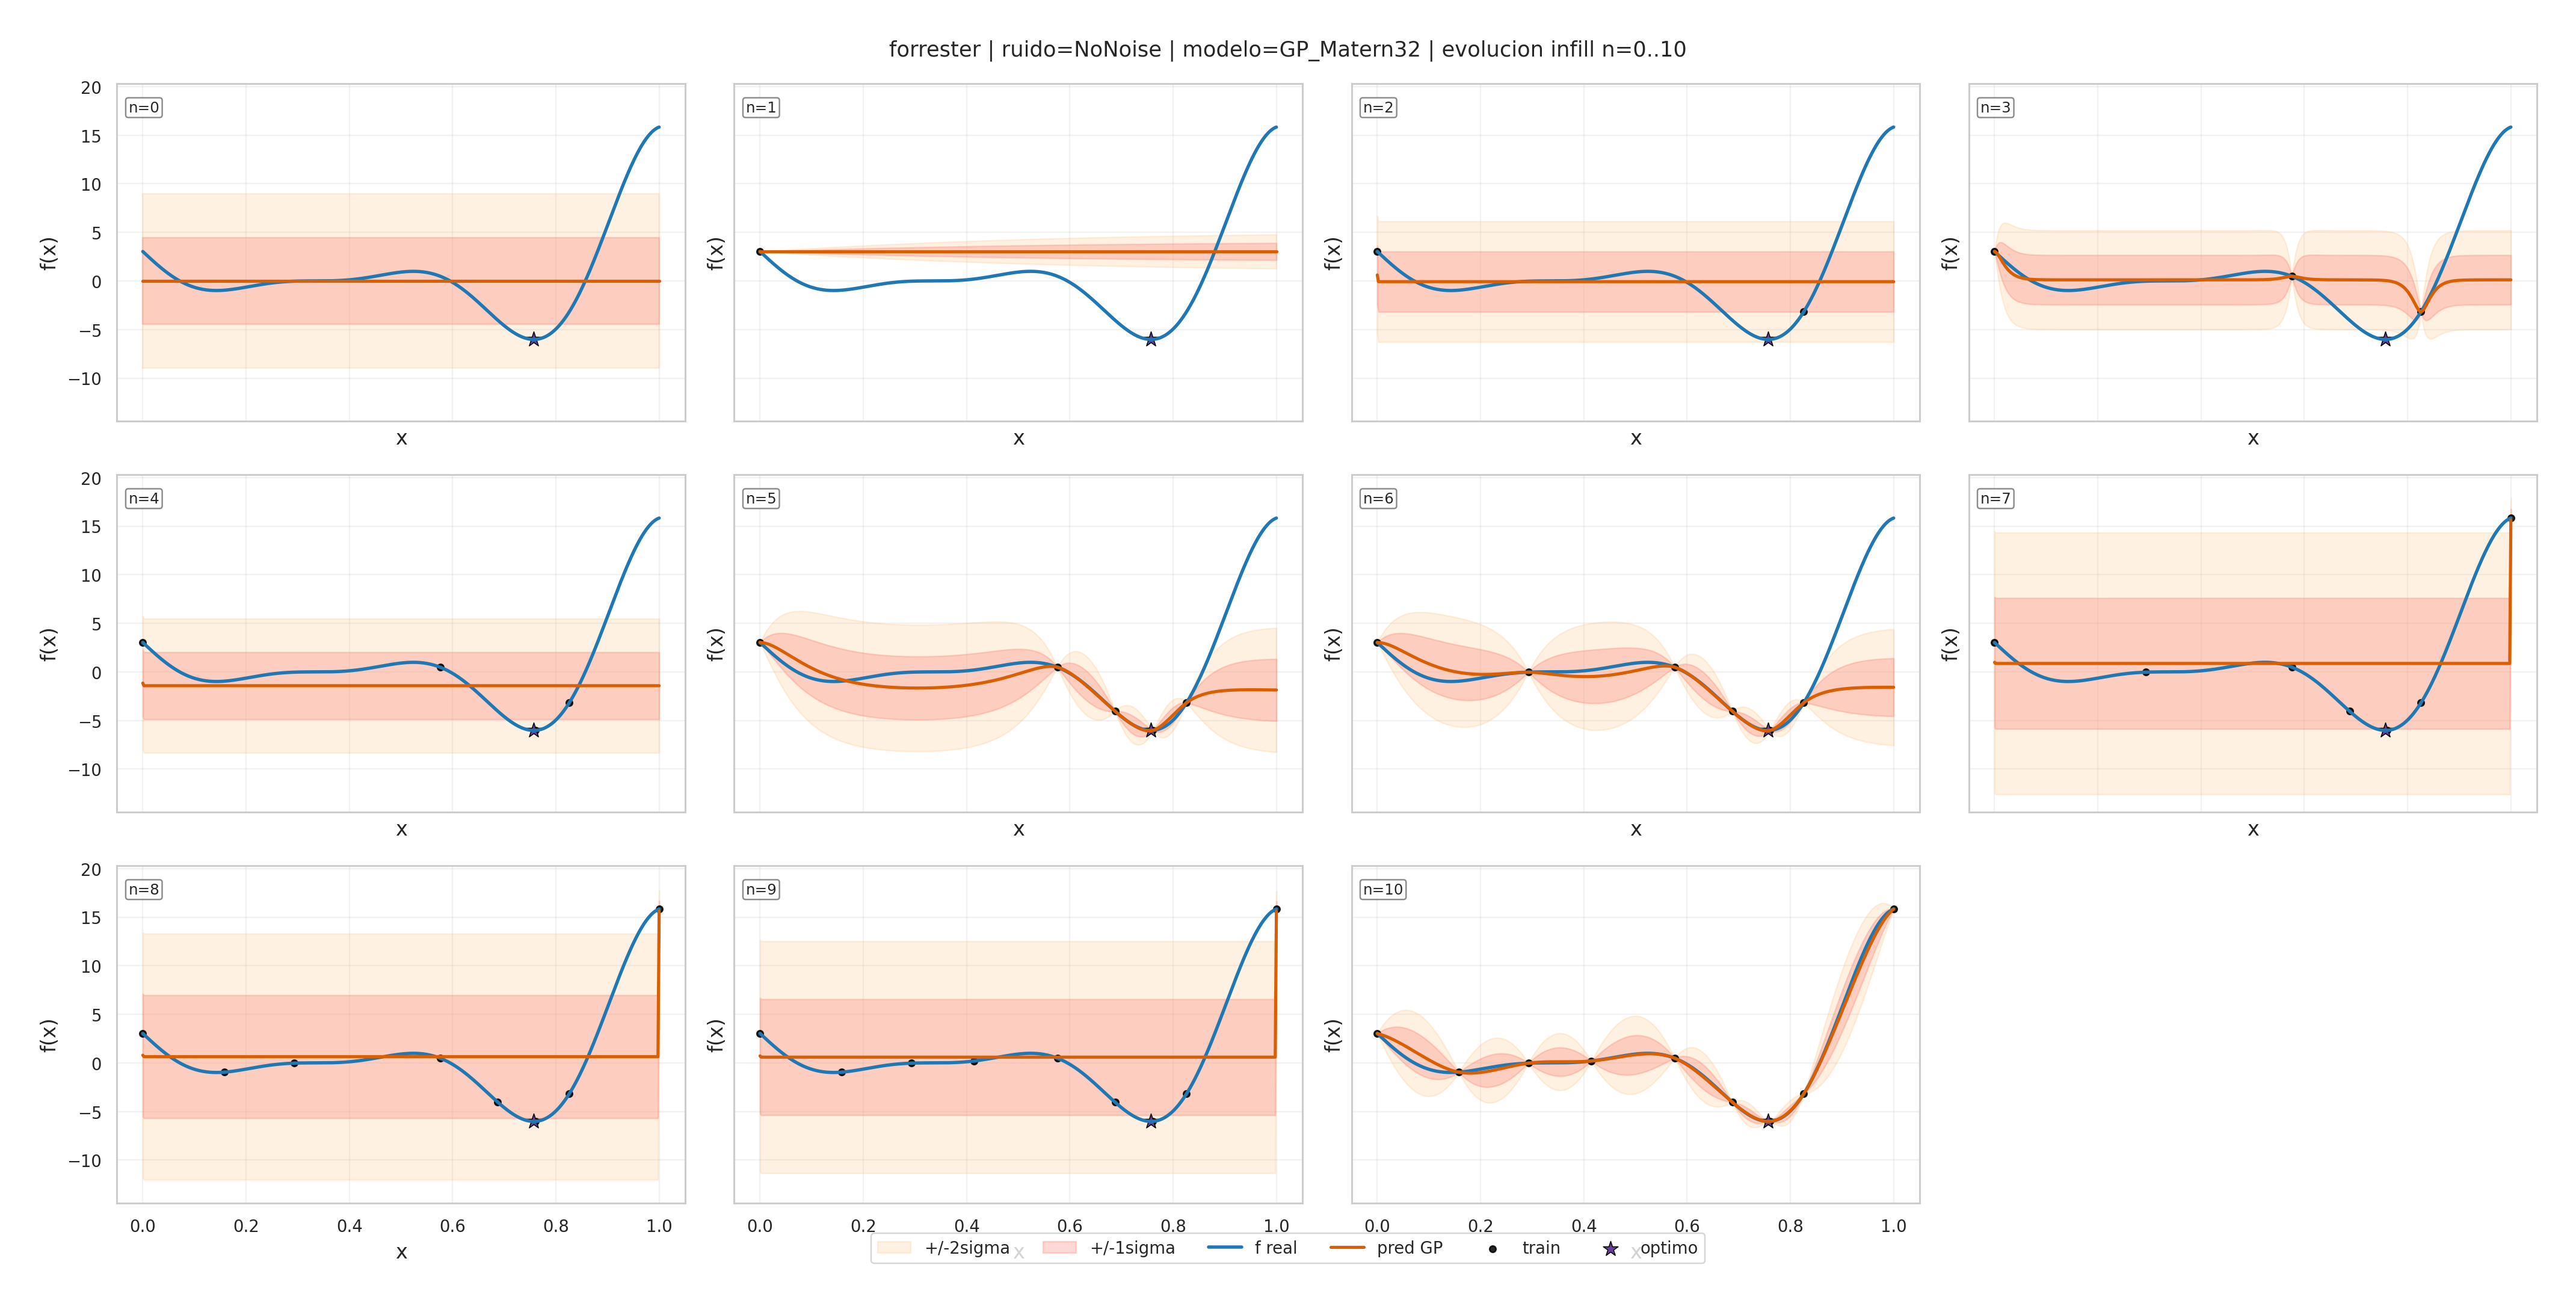
\includegraphics[width=\textwidth]{assets/app_forrester_gp_evolution_no_noise.png}
\caption[Evaluación del proceso de infill en Forrester]{Evolución del proceso de \emph{infill} en Forrester sin ruido. Cada panel muestra el estado del GP tras incorporar un número creciente de puntos. La línea azul representa la función real, la línea naranja la media predictiva del GP, las bandas muestran la incertidumbre y los puntos indican las observaciones disponibles.}
\label{fig:app_forrester_gp_evolution_no_noise}
\end{figure}
\FloatBarrier

La Figura~\ref{fig:app_forrester_gp_evolution_no_noise} permite observar cómo el modelo sustituto cambia a medida que se incorporan nuevas observaciones. En las primeras iteraciones, la incertidumbre domina grandes zonas del dominio. Conforme el proceso avanza, el modelo ajusta mejor la región cercana al mínimo y reduce la incertidumbre alrededor de los puntos evaluados. Esta visualización ayuda a interpretar por qué el proceso no debe evaluarse solo mediante MAE: una predicción global imperfecta puede seguir siendo útil si orienta la búsqueda hacia regiones prometedoras.

\section{Decisión puntual mediante Expected Improvement}
\label{app:forrester_ei_decision}

La Figura~\ref{fig:app_forrester_ei_decision_synthesis} muestra una decisión concreta de EI en Forrester. El GP se entrena con cuatro puntos iniciales de Sobol y varias evaluaciones de \emph{infill} previas. En el paso representado, EI propone el siguiente punto en \(x_{\mathrm{next}}=0.763\), muy cercano al óptimo conocido del benchmark.

\begin{figure}[htbp]
\centering
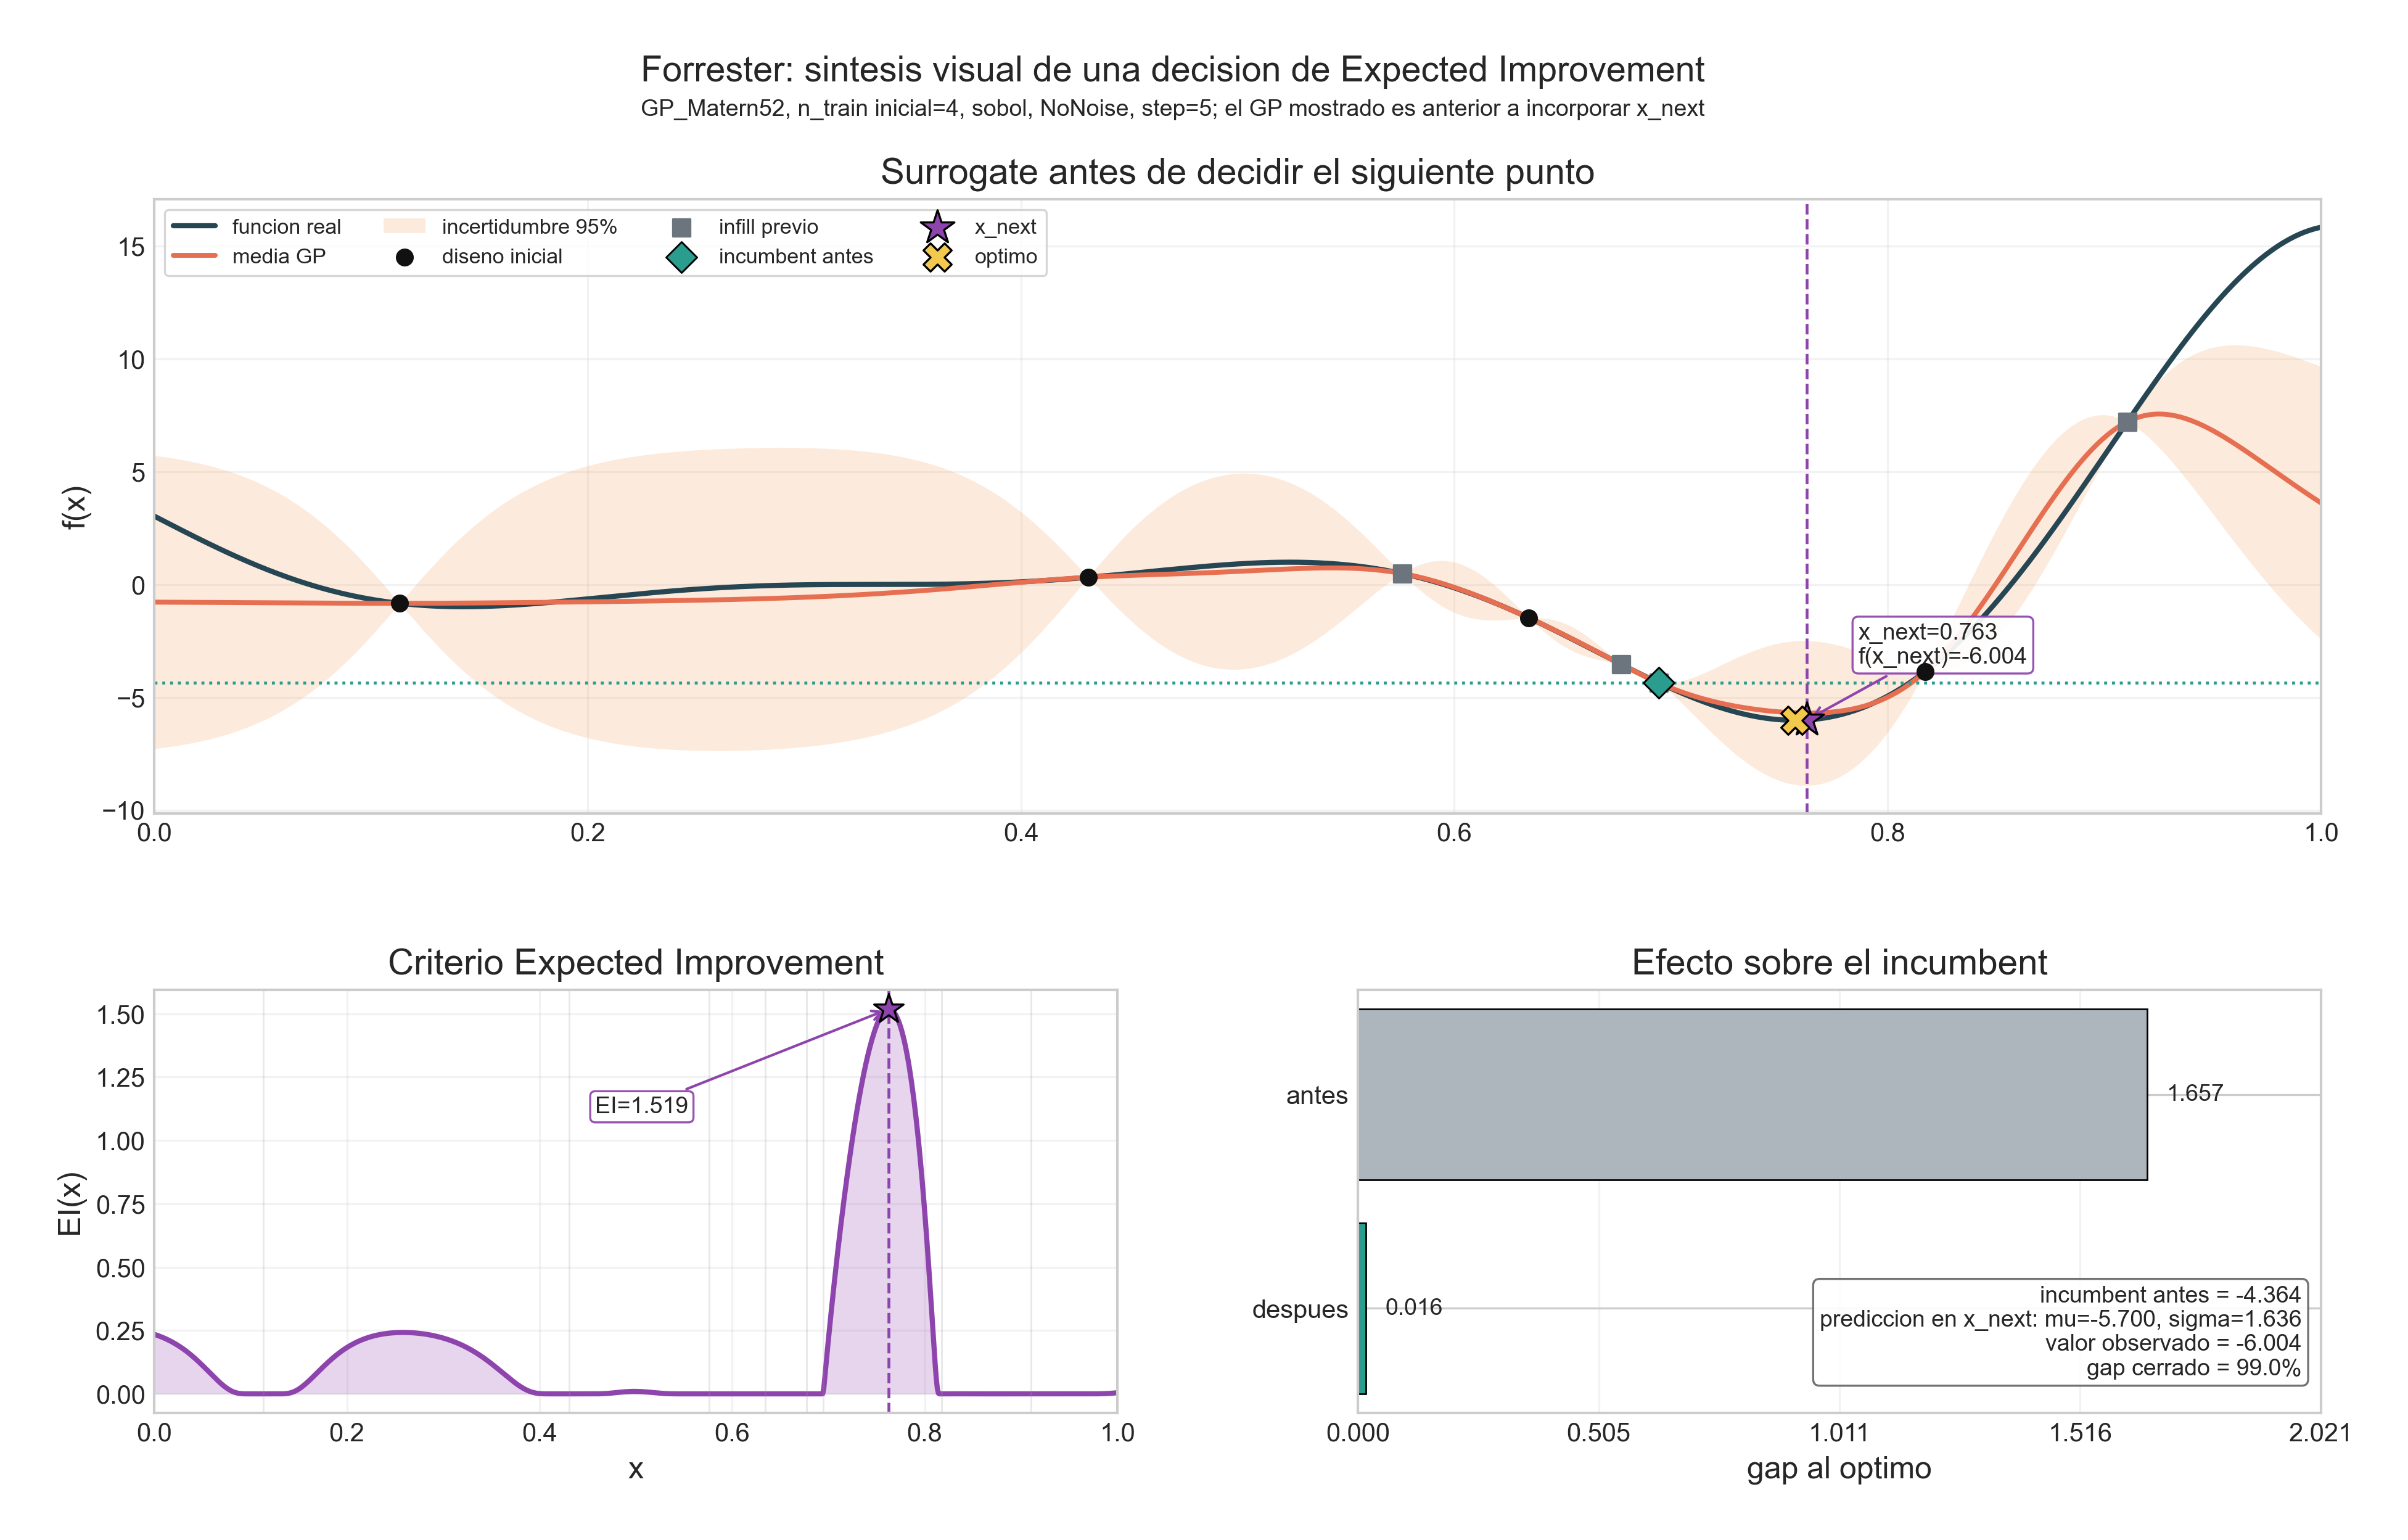
\includegraphics[width=\textwidth]{assets/app_forrester_ei_decision_synthesis_step5.png}
\caption[Proceso de decisión mediante EI en Forrester]{Síntesis visual de una decisión de Expected Improvement en Forrester. El panel superior muestra la media posterior, la incertidumbre, las observaciones previas, el \emph{incumbent} y el punto propuesto. El panel inferior izquierdo representa la función de adquisición EI, y el panel inferior derecho cuantifica el cambio en el gap al óptimo tras evaluar el nuevo punto.}
\label{fig:app_forrester_ei_decision_synthesis}
\end{figure}

\begin{table}[htbp]
\centering
\small
\caption[Decisión EI en Forrester]{Resumen numérico de la decisión EI representada en la Figura~\ref{fig:app_forrester_ei_decision_synthesis}.}
\label{tab:app_forrester_ei_decision}
\renewcommand{\arraystretch}{1.15}
\begin{tabularx}{\textwidth}{@{}p{4.5cm} X@{}}
\toprule
\textbf{Elemento} & \textbf{Valor} \\
\midrule
Benchmark & Forrester \\
Modelo & GP\_Matern52 \\
Diseño inicial & Sobol, \(n_{\mathrm{train}}=4\), sin ruido \\
Paso de \emph{infill} & 5 \\
Punto propuesto & \(x_{\mathrm{next}}=0.763\) \\
EI en el punto propuesto & 1.519 \\
Mejor valor observado antes & -4.364 \\
Valor observado en \(x_{\mathrm{next}}\) & -6.004 \\
Óptimo conocido & \(f(x^\star)=-6.021\) \\
Gap cerrado tras la evaluación & 99.0 \% \\
\bottomrule
\end{tabularx}
\end{table}
\FloatBarrier
Este ejemplo muestra el papel práctico de la incertidumbre en un GP. EI no selecciona un nuevo punto solo por la media predicha, sino por la combinación entre mejora esperada y dispersión predictiva. En este caso, el punto elegido queda muy cerca del óptimo real y reduce casi por completo el gap que existía antes de la evaluación.

\section{Contrastes estadísticos complementarios}
\label{app:contrastes_infill_benchmarks}

Además de las tablas descriptivas, los registros generados por el experimento permiten realizar contrastes no paramétricos sobre los resultados de los benchmarks. Estos contrastes no se plantean como una demostración formal de superioridad universal, sino como una comprobación complementaria de dos efectos observados en el análisis principal: la mejora del \emph{incumbent} durante el proceso de \emph{infill} y la existencia de diferencias entre familias de kernels GP.

Para evaluar la mejora del \emph{incumbent}, se comparó el mejor valor observado al inicio y al final de cada trayectoria activa. Cada trayectoria queda definida por benchmark, muestreador, tamaño inicial, configuración de ruido, modo de validación y modelo. Dado que la función objetivo de los benchmarks se formula como minimización, una reducción del \emph{incumbent} indica mejora. El Cuadro~\ref{tab:app_wilcoxon_infill_incumbent} resume un contraste de rangos con signo de Wilcoxon unilateral, con alternativa de mejora tras el proceso de \emph{infill}.

\begin{table}[htbp]
\centering
\small
\caption[Contraste de mejora del incumbent]{Contraste de mejora del \emph{incumbent} entre el inicio y el final de las trayectorias de \emph{infill}.}
\label{tab:app_wilcoxon_infill_incumbent}
\renewcommand{\arraystretch}{1.15}
\begin{tabularx}{\textwidth}{@{}X r r r r@{}}
\toprule
\textbf{Modelo} & \textbf{Trayectorias} & \textbf{Mejoran} & \textbf{Mediana mejora} & \textbf{\(p\)-valor} \\
\midrule
Todos los GP & 372 & 316 & 2.812 & \(7.35\times10^{-54}\) \\
GP\_Linear & 66 & 30 & 0.000 & \(8.67\times10^{-7}\) \\
GP\_Matern32 & 66 & 62 & 2.970 & \(3.79\times10^{-12}\) \\
GP\_Matern52 & 66 & 60 & 2.519 & \(8.15\times10^{-12}\) \\
GP\_Matern52\_ARD & 54 & 54 & 8.105 & \(8.13\times10^{-11}\) \\
GP\_RBF & 66 & 59 & 2.574 & \(1.20\times10^{-11}\) \\
GP\_RBF\_ARD & 54 & 51 & 7.602 & \(2.57\times10^{-10}\) \\
\bottomrule
\end{tabularx}
\end{table}
\FloatBarrier

Los resultados muestran que el proceso de \emph{infill} reduce el \emph{incumbent} de forma sistemática en las trayectorias consideradas. El efecto es especialmente claro en los kernels con ARD y en los kernels Matérn/RBF, mientras que el modelo lineal presenta una mejora mediana nula, aunque sin empeorar en muchas configuraciones y con mejoras puntuales suficientes para que el contraste agregado sea significativo.

Para comparar los kernels GP en términos predictivos, se utilizó el MAE de los bloques completos compartidos por todos los kernels. Cada bloque corresponde a una combinación de benchmark, muestreador, tamaño inicial, configuración de ruido y modo de validación. Sobre los 54 bloques completos, el test de Friedman detecta diferencias entre modelos \((p=1.88\times10^{-6})\). El Cuadro~\ref{tab:app_friedman_kernels_gp} muestra los rangos medios y los contrastes pareados de Wilcoxon frente al kernel con mejor rango medio.

\begin{table}[htbp]
\centering
\small
\caption[Contraste entre kernels GP en benchmarks]{Comparación no paramétrica entre kernels GP usando el MAE en bloques completos. Rangos menores indican mejor comportamiento.}
\label{tab:app_friedman_kernels_gp}
\renewcommand{\arraystretch}{1.15}
\begin{tabularx}{\textwidth}{@{}l r r X@{}}
\toprule
\textbf{Modelo} & \textbf{Rango medio} & \textbf{\(p\) vs. GP\_Matern52\_ARD} & \textbf{Lectura} \\
\midrule
GP\_Matern52\_ARD & 2.741 & -- & Mejor rango medio. \\
GP\_RBF\_ARD & 2.815 & 0.677 & Rendimiento prácticamente indistinguible del mejor. \\
GP\_Matern52 & 3.370 & \(4.51\times10^{-4}\) & Peor que la versión ARD en el contraste pareado. \\
GP\_RBF & 3.593 & 0.138 & Diferencia no concluyente frente al mejor. \\
GP\_Matern32 & 4.056 & \(2.04\times10^{-5}\) & Peor que el mejor kernel en los bloques compartidos. \\
GP\_Linear & 4.426 & \(5.28\times10^{-8}\) & Menor rendimiento predictivo agregado. \\
\bottomrule
\end{tabularx}
\end{table}
\FloatBarrier

Estos contrastes apoyan dos conclusiones utilizadas en la memoria: primero, el ciclo de \emph{infill} aporta mejora efectiva sobre el mejor valor observado; segundo, los kernels con ARD tienden a ocupar las mejores posiciones en MAE. Sin embargo, no se observa una separación estadística clara entre GP\_Matern52\_ARD y GP\_RBF\_ARD, por lo que la elección de un kernel concreto debe interpretarse junto con la estabilidad, el coste computacional y el comportamiento en cada problema.
